\documentclass[10pt,a4paper]{article}
\usepackage[utf8x]{inputenc}
\usepackage{ucs}
\usepackage[spanish]{babel}
\usepackage{amsmath}
\usepackage{amsfonts}
\usepackage{amssymb}
\usepackage{makeidx}
\usepackage{graphicx}
\usepackage{lmodern}
\usepackage{kpfonts}
\usepackage{float}
\usepackage{tikz}
\def\firstcircle{(90:1.75cm) circle (1.5cm)}
\def\secondcircle{(210:1.75cm) circle (1.5cm)}
\def\thirdcircle{(330:1.75cm) circle (1.5cm)}

\usepackage[left=2cm,right=2cm,top=2cm,bottom=2cm]{geometry}
%\begin{document}

\headsep17mm
\topmargin-1cm
\hoffset -1.5cm \voffset -1cm \textwidth 17cm \oddsidemargin
1.5cm \evensidemargin 1.5cm \textheight 22.5cm

\newcommand{\coef}[2]{\left( \begin{array}{c} #1 \\ #2 \end{array}\right)}
\newcommand{\atr}{\hspace{-0,12cm}}
%\newcommand{\atrs}{\hspace{-0,1cm}}


\newcommand{\en}{\subset}
\newcommand{\inte}[1]{#1^{(int)}}

\newcommand{\N}{\mbox{$\mathbb{N}$}}
\newcommand{\Z}{\mbox{$\mathbb{Z}$}}
\newcommand{\Q}{\mbox{$\mathbb{Q}$}}
\newcommand{\R}{\mbox{$\mathbb{R}$}}
\newcommand{\K}{\mbox{$\mathbb{K}$}}
\newcommand{\exte}[1]{#1^{(ext)}}
\newcommand{\sgn}{{\rm sgn\,}}
\newcommand{\bi}{\begin{itemize}}
\newcommand{\ei}{\end{itemize}}
\newcommand{\esp}{\vspace*{3mm}}
\newcommand{\uno}{\vspace*{1cm}}
\newcommand{\pirulo}[1]{\mbox{$#1^{^{^{\!\!\!\!\!\!\!\!\!\longrightarrow}=}}$}}
\newcommand{\Po}[1]{\mbox{${\cal P}_{#1}$}}
\newcommand{\M}[2]{\mbox{${\cal M}(\R)_{#1x#2}$}}
\newcommand{\MC}[2]{\mbox{${\cal M}(\C)_{#1x#2}$}}
\newcommand{\C}{\mbox{\mathbb{C}}}
\newcommand{\noin}{\mbox{$\in\!\!\!\!/$}}
\newcommand{\cla}[1]{\overline{#1}}
\newcommand{\dem}{{\sc Demostraci\'{o}n.}}
\newcommand{\al}{\alpha}
\newcommand{\itm}[1]{\item [(#1)]}
\newcommand{\eps}{\epsilon}
\newcommand{\conj}{$\left\{\ /\ \right\}$}
\newcommand{\imp}{\int_a^{+\infty} f}
\newcommand{\gral}{\int_a^x f}
\newcommand{\valo}{[a,b]}
\newcommand{\reg}{{\cal R}\left( f,[a,b] \right)}
\newcommand{\chiri}{$\spadesuit$}


\newcommand{\tend}[1]{\mathop{\longrightarrow} \limits_{#1}}
\newcommand{\tends}[2]{\mathop{\longrightarrow} \limits_{#1 \to #2}}
\newcommand{\mifrac}[2]{\frac{{\textstyle #1}}{{\textstyle #2}}}
\newcommand{\milim}[2]{\mathop{\rm lim} \limits_{#1 \to #2}}
\newcommand{\integ}[3]{\int \limits_{#1}^{#2} #3}
\newcommand{\integdx}[3]{\int \limits_{#1}^{#2} #3 \, dx}
\newcommand{\integdt}[3]{\int \limits_{#1}^{#2} #3 \, dt}
\newcommand{\integdu}[3]{\int \limits_{#1}^{#2} #3 \, du}
\newcommand{\integdy}[3]{\int \limits_{#1}^{#2} #3 \, dy}
\newcommand{\dosfilas}[2]{\mathop{}
  \limits_{{\scriptstyle #2}}^{{\scriptstyle #1}}}
\newcommand{\dosfilasnormales}[2]{\mathop{}
  \limits_{{\textstyle #2}}^{{\textstyle #1}}}
\newcommand{\deffun}[4]{\left\{ \begin{array}{ccl} #1 & \mbox{si} & #2 \\ #3 & \mbox{si} & #4 \end{array} \right.}
\newcommand{\deffunoc}[3]{\left\{ \begin{array}{cl} #1 & \,\, \mbox{si} \,\,\, #2 \\ #3 & \,\, \mbox{en otro caso} \end{array} \right.}
\newcommand{\deffuntres}[6]{\left\{ \begin{array}{ccl} #1 & \mbox{si} & #2 \\ #3 & \mbox{si} & #4 \\ #5 & \mbox{si} & #6 \end{array} \right.}
\newcommand{\deffunoctres}[5]{\left\{ \begin{array}{cl} #1 & \,\, \mbox{si} \,\,\, #2 \\ #3 & \,\, \mbox{si} \,\,\, #4 \\ #5 & \,\, \mbox{en otro caso} \end{array} \right.}
\newcommand{\sistdos}[2]{\left \{ \begin{array}{l} #1 \\ #2 \end{array} \right.}

\newcounter{cuent}
\newcommand{\proba}[1]{\stepcounter{cuent}{\alph{cuent})\quad}
\displaystyle#1\qquad}
\newcommand{\cuento}{\setcounter{cuent}{0}}

\begin{document}
\noindent {\bf Facultad de Ingeniería - Tecnólogo en informática}
\hfill {\bf Matemática discreta y Lógica 1} \\
       {\bf Primer semestre 2018}

\vspace{0,3cm}

\begin{center}
{\bf \Large Pr\'actico 1}
\end{center}

\vspace{0,3cm}

\section{Conjuntos}

\begin{enumerate}

\item Determinar cuantos subconjuntos de $A = \{1,2,a,b,c \}$ tienen 2 elementos. Repetir lo mismo para 3 elementos.

\item Sean $A$, $B$ y $C$ los conjuntos dados por $A=\{1,2,3,4,5\}$, $B=\{3,4,5,6,7\}$ y $C= \{7,8,9\}$

Calcular:
$$\proba{ A \cap B } \proba{ B \cap C } \proba{ A \cap C }  \proba{ A \cap B \cap C }$$
$$ \proba{ A \cup B } \proba{ B \cup C } \proba{ A \cup C }  \proba{ A \cup B \cup C } \proba{ A \cup (B \cap C ) } \proba{ A \cap (B \cup C ) }$$
$$  \proba{ (A \setminus B) \cup   (B \setminus A)} \proba{ (A \setminus C) \cup   (C \setminus A)} \proba{ A \cup (B \setminus C) } $$
\cuento

\item Determinar todos los elementos de los siguientes conjuntos:
$$\proba{ \{ n \in \N : n \leq 5 \} }  \proba{ \{n \in \N: n^{2} \leq 12 \}} \proba{ \left\lbrace(-1)^{n} : n \in \N\right\rbrace } \proba{ \{ x \in \R : x^{2} - x + 2 = 0 \} }$$\cuento


\item Sean $A$, $B$ y $C$ tres conjuntos como en la figura:

\begin{figure}[H]
\centering
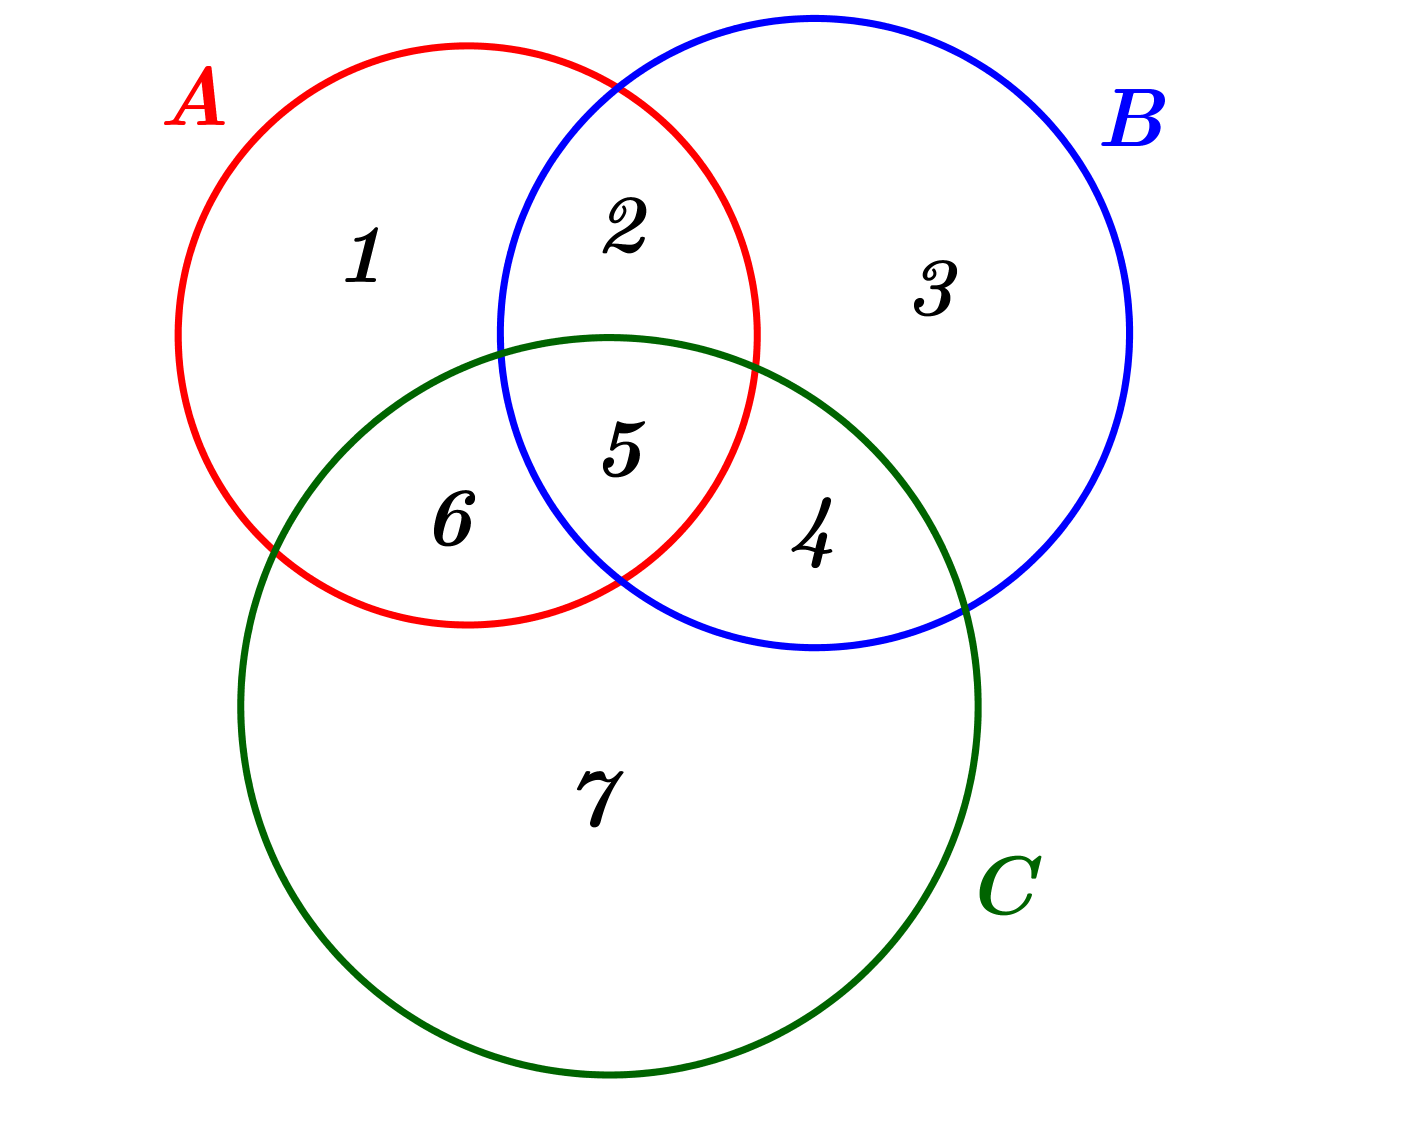
\includegraphics[scale=0.5]{diagramavenn1.png}
\end{figure}

Describir las regiones numeradas a partir de los conjuntos $A$, $B$ y $C$ y las operaciones binarias $\cup$, $\cap$ y $\setminus$.

\item Sean $A$ y $B$ dos conjuntos finitos. Ordene los siguientes conjuntos
  según la cantidad de elementos que tengan, en forma creciente:
$$A,\,\,\, A \cap B,\,\,\, A \cup B,\,\,\, \emptyset,\,\,\, A \cup (B \setminus A)$$


\item Determinar cuáles de las siguientes igualdades e inclusiones son verdaderas o falsas. En caso de que una igualdad sea falsa determinar si se da alguna de las inclusiones.
$$\proba{ A \cup (B \cup C)  = (A \cup B) \cup C}  \proba{ A \cap (B \cap C)  = (A \cap B) \cap C} \proba{ (A \cup B) \cap A  = A \cup (B \cap A)}  $$
$$ \proba{ A \cup (B \cap C) = (A \cup B) \cap (A \cup C)}  \proba{ A \cap (B \cup C) = (A \cap B) \cup (A \cap C)}   $$\cuento


\item Determinar cuáles de las siguientes igualdades e inclusiones son verdaderas o falsas. En caso de que una igualdad sea falsa determinar si se da alguna de las inclusiones.
$$ \proba{ A \setminus ( B \setminus A) = \emptyset } \proba{ (A \setminus  B)  \setminus A = \emptyset }  \proba{[A \setminus B] = [A \setminus (A \cap B) ]}  $$
$$\proba{ A \setminus (A \setminus B) = B } \proba{ [A \cap (B \setminus C)] = [(A \cap B ) \setminus (A \cap C)] }  \proba{[A \cap (B \setminus C)] = [(A \cap B) \setminus C ] } $$
$$\proba{ A \setminus (B \cup C) = [(A \setminus B) \cup (A \setminus C)] } \proba{ A \setminus (B \cup C) = [(A \setminus B) \cap (A \setminus C)] }  $$
\cuento

\item { \bf Producto cartesiano }

En este ejercicio todos los conjuntos considerados son no vac\'ios.
\begin{enumerate}
\item Sean $A = \{1,2,3\}$ y $B=\{a,b,c\}$. Listar todos los elementos de $A \times B$ y de $B \times A$.

\item Sean $A$ y $B$ dos conjuntos cualesquiera. Probar que si $(x,y) \in A \times B$ y adem\'as $(x,y) \in B \times A$ entonces $\{x,y\} \subset A \cap B$.

\item Probar que si $A \times B = B \times A$ entonces $A = B$.
\end{enumerate}

\item Bosquejar en un par de ejes coordenados (es decir, en  $\R \times \R$),
  los siguientes conjuntos:
$$\proba{ A = \{ (x,y) \in \R\times \R : y = 2\} } \proba{ B = \{ (x,y) \in \R\times \R : x = -3 \} } \proba{C = \{ (x,y) \in \R\times \R : x = y\}} $$ \cuento


\end{enumerate}

\end{document}
